\documentclass{standalone}
\usepackage[T1]{fontenc}
\usepackage[utf8]{inputenc}
\usepackage{pgf,tikz}
\usepackage{setspace}
\usepackage{pgfplots}
%\pgfplotsset{compat=1.9}


\begin{document}


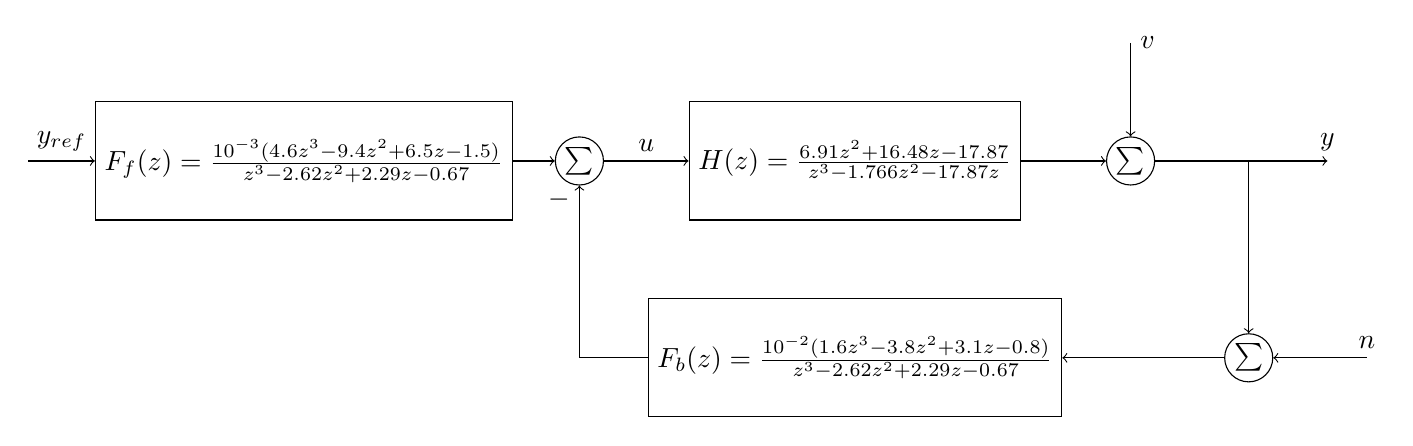
\begin{tikzpicture}[
    node distance=2cm, block/.style={rectangle, draw, minimum height=15mm, minimum width=20mm}, sumnode/.style={circle, draw, inner sep=1pt}]

  \node[coordinate] (input) {};
  \node[block, right of=input, node distance=35mm] (TR) {$F_f(z)=\frac{10^{-3}(4.6z^3 - 9.4z^2 + 6.5z - 1.5)}{z^3 - 2.62z^2 + 2.29z - 0.67}$};
  \node[sumnode, right of=TR, node distance=35mm] (sum) {$\sum$};
  \node[block,right of=sum, node distance=35mm] (plant) {$H(z)=\frac{6.91z^2 + 16.48z - 17.87}{z^3 - 1.766z^2 - 17.87z}$};
  \node[sumnode, right of=plant, node distance=35mm] (sumdist) {$\sum$};
  \node[coordinate, above of=sumdist, node distance=15mm] (dist) {};
  \node[coordinate, right of=sumdist, node distance=15mm] (measure) {};
  \node[coordinate, right of=measure, node distance=10mm] (output) {};
  \node[block,below of=plant, node distance=25mm] (SR) {$F_b(z)=\frac{10^{-2}(1.6z^3 - 3.8z^2 + 3.1z - 0.8)}{z^3 - 2.62z^2 + 2.29z - 0.67}$};
  \node[sumnode,below of=measure, node distance=25mm] (sumnoise) {$\sum$};
  \node[coordinate, right of=sumnoise, node distance=15mm] (noise) {};

  \draw[->] (input) -- node[above] {$y_{ref}$} (TR);
  \draw[->] (TR) -- node[above] {} (sum);
  \draw[->] (sum) -- node[above] {$u$} (plant);
  \draw[->] (plant) -- (sumdist);
  \draw[->] (dist) -- node[at start, right] {$v$} (sumdist);
  \draw[->] (sumdist) -- node[at end, above] {$y$} (output);
  \draw[->] (measure) -- (sumnoise);
  \draw[->] (noise) -- node[at start, above] {$n$} (sumnoise);
  \draw[->] (sumnoise) -- (SR);
  \draw[->] (SR) -| (sum) node[left, pos=0.96] {$-$};

\end{tikzpicture}
\end{document}


